% P5 manuscript — target: Journal of Cheminformatics (Springer Nature)
\documentclass[11pt,a4paper]{article}

\usepackage[margin=1in]{geometry}
\usepackage{amsmath,amssymb}
\usepackage{authblk}
\usepackage{booktabs}
\usepackage{graphicx}
\graphicspath{{../results/figures/}}
\usepackage{hyperref}
\usepackage{microtype}
\usepackage[numbers,sort&compress]{natbib}
\usepackage{xcolor}
\usepackage{siunitx}
\sisetup{
  detect-all           = true,
  group-minimum-digits = 4,
  range-phrase         = {--},
  range-units          = single,
}
\usepackage[nameinlink,noabbrev]{cleveref}

\title{\textbf{Do larger molecular models improve antimalarial activity prediction? A scaffold-controlled comparison with ECFP4}}

\author[1]{Myke Vital Sao Temgoua\thanks{Corresponding author: myke-vital.sao@facsciences-uy1.cm}}
\author[1]{Jean-Pierre Tchapet Njafa}
\author[1]{Serge Guy Nana Engo}
\author[2]{Penabei Samafou}
\author[3]{Wilfred Fon Mbacham}

\affil[1]{Department of Physics, Faculty of Science, University of Yaound\'e I, P.O. Box 812, Yaound\'e, Cameroon}
\affil[2]{Department of Medical Imaging and Radiation Sciences, Universit\'e de Sherbrooke, Sherbrooke, QC, Canada}
\affil[3]{Department of Biochemistry, Faculty of Science, University of Yaound\'e I, P.O. Box 812, Yaound\'e, Cameroon}

\date{\today}

\begin{document}

\maketitle

\begin{abstract}
On a curated antimalarial natural-product panel, do graph neural networks and pretrained sequence transformers improve activity ranking beyond a compact ECFP4--random-forest baseline when chemical scaffolds are held out? We benchmark ECFP4--RF against a graph isomorphism network (GIN), two topological fusion variants (GIN--TFP and GIN--TNE), and a fine-tuned ChemBERTa transformer on \num{19836} African antimalarial natural products using random and Bemis--Murcko scaffold five-fold cross-validation (\num{25} fold--seed replicates). Under the scaffold split, ECFP4--RF achieves ROC AUC \num{0.8300}; every neural arm is significantly worse after Benjamini--Hochberg correction (GIN--TFP \num{0.8138}, GIN--TNE \num{0.8090}, GIN \num{0.8047}, ChemBERTa \num{0.7867}). Persistent-image dimensions carry the largest fusion-head salience, indicating that topological features carry geometric signal even though they do not improve ranking. These results establish a controlled benchmark on an antimalarial natural-product panel and caution against assuming that model scale improves out-of-distribution prediction for this chemical class.
\end{abstract}

\textbf{Contribution:} We provide a controlled benchmark showing that ECFP4--RF remains the strongest tested predictor on an antimalarial natural-product panel under scaffold separation, while topological fusion supplies descriptive geometric signal without improving ranking. The study also specifies fold-independent initialization for the pretrained transformer, a necessary condition for valid cross-validation.

\noindent\textbf{Keywords:} graph neural networks; molecular fingerprints; antimalarial natural products; scaffold split; benchmark; interpretability; persistent homology

\noindent\textbf{Highlights:}
\begin{itemize}
\item Under the scaffold split, ECFP4--RF (AUC \num{0.8300}) outperforms every GNN/transformer arm; all arms are significantly worse (BH-adjusted $p \le \num{0.0378}$)
\item Fold-independent transformer initialization changes the apparent ranking of sequence models and is required for valid cross-validation
\item Persistent-image dimensions have the largest descriptive projection-weight salience in the topological fusion head
\item Reproducible frozen splits (random + scaffold), \num{25} fold--seed replicates per split, and released checkpoints
\end{itemize}

\section{Introduction}

Malaria remains a leading infectious disease burden in sub-Saharan Africa, with \num{247} million cases and \num{619000} deaths in \num{2023} \citep{who2024malariareport}. Control is increasingly threatened by the emergence of artemisinin-resistant \emph{Plasmodium falciparum} strains in Southeast Asia and Africa \citep{ariyey2014,ashley2018}, prompting an urgent, WHO-endorsed need for new scaffolds that remain active against drug-resistant parasites. African natural products (NPs) constitute a rich source of chemically diverse scaffolds \citep{anpdb_2026,value_addition_african_np_2025}. The panel studied here descends from a screening campaign seeded on \num{396} African NP and \num{454} synthetic-drug scaffolds \citep{temgoua2026antimalarial}; separate molecular-dynamics work in the same research programme examined selected leads against resistance-associated targets and mutations \citep{temgoua2027md}. Computational screening of NP libraries promises to accelerate hit identification in this resistance-driven search, yet the cheminformatics representation strongly conditions the outcome. In recent years, a ``scale-centric'' narrative has emerged in molecular machine learning: pretrained molecular foundation models and sequence transformers are expected to supersede compact, task-trained cheminformatics models \citep{mol_tdl_2026,tn_efficient_2026}. This narrative extends to quantum-inspired representations, where quantum computing is increasingly discussed as a paradigm for drug discovery and bioinformatics \citep{naleczcharkiewicz2024,kumar2024quantumdrug}.

This narrative is increasingly challenged by rigorous, controlled benchmarks. In a \num{156}-comparison benchmark across \num{26} endpoints, Guo and Ding found that classical machine learning on fingerprints wins \qty{47.4}{\percent} of task--metric entries, ahead of pretrained sequence models (\qty{28.8}{\percent}) and GNNs (\qty{21.8}{\percent}), with the classical advantage largest under random splits and shrinking, but not vanishing, under scaffold-separated protocols \citep{guo_ding_2026}. An independent comparison of \num{25} pretrained embedding models across \num{25} datasets found that \emph{almost no neural embedding statistically improves over the ECFP fingerprint baseline} \citep{benchmark_pretrained_2025}. And for natural products specifically, a \num{20}-fingerprint benchmark over \num{100000}+ NPs showed that no single encoding dominates, and that ECFP is frequently matched or exceeded by alternative fingerprints on NP bioactivity tasks \citep{boldini2024}.

Three questions determine whether this conclusion is informative: do the findings extend to a dedicated antimalarial natural-product panel with high structural complexity; do persistent-homology and tensor-network descriptors add value inside a GNN fusion architecture under scaffold separation; and does fold-independent initialization alter the apparent performance of a pretrained transformer?

\subsection{Related work}

The tension between classical cheminformatics and neural molecular learning has been documented across multiple benchmarks. For molecular property prediction, random forests on ECFP fingerprints remain competitive with or superior to GNNs on small-to-medium datasets ($<$ \num{10000} molecules) \citep{guo_ding_2026,benchmark_pretrained_2025}. GNN architectures (GCN, GAT, GIN) have shown gains on large, curated datasets such as MoleculeNet \citep{wu_molnet_2018}, but these gains often diminish under scaffold splits that better reflect real-world drug discovery \citep{guo_ding_2026}. Pretrained sequence transformers (ChemBERTa, MolBERT) leverage large unlabeled corpora but have shown inconsistent gains on downstream tasks, particularly when the target dataset is structurally dissimilar to the pretraining data \citep{chemberta_2020,benchmark_pretrained_2025}.

Topological data analysis (TDA) has been applied to molecular representation through persistent homology, producing descriptors that capture ring systems, molecular cavities, and higher-order connectivity \citep{tda_review_2025}. Recent work has fused TDA features with GNN architectures, reporting modest improvements on specific tasks \citep{topology_molecular_representations_2025}. Multimodal fusion of graph and sequence representations---for example, concatenating GCN embeddings with ChemBERTa latent vectors---has shown promise on small datasets \citep{rollins2024molprop}. More broadly, computational MoA analyses emphasize that chemical, phenotypic, and network data capture complementary biological levels; target prediction alone is therefore not equivalent to a complete mechanism assignment \citep{Trapotsi2022MoA}. Tensor-network embeddings, derived from Tucker decomposition of molecular tensors, provide compressed representations that retain scaffold-relevant information \citep{tn_efficient_2026}. However, neither TDA nor tensor-network features have been systematically tested inside GNN fusion architectures under rigorous scaffold-split protocols on antimalarial panels.

We therefore benchmark GIN, GIN--TFP, GIN--TNE, and ChemBERTa against ECFP4--RF under both random and scaffold splits. We test three linked questions: whether learned models exceed ECFP4, whether topological fusion narrows the scaffold gap, and whether projection-weight salience identifies a reproducible geometric signal even when ranking does not improve. The comparison is designed to distinguish predictive performance from interpretability and to quantify the effect of fold-independent transformer initialization.

\section{Results}

\subsection{Baseline and evaluation question: a reproducible reference for model comparison}

To verify reproducibility, we independently reproduced the ECFP4--RF baseline reported for the same molecular collection \citep{temgoua2027quantum}. Under the random split we obtain $\num{0.9433} \pm \num{0.0003}$ across five per-seed means (range \num{0.9428}--\num{0.9437}), compared with the reference value of $\num{0.9475} \pm \num{0.0045}$. The difference is compatible with the distinct frozen split and random-seed realization used here, supporting comparability of the panel and fingerprint implementation.

\subsection{H1: scaffold-held-out prediction favours ECFP4 over learned representations}

\begin{table}[t]
\centering
\caption{Mean test ROC AUC $\pm$ SD of the five per-seed means (each seed averages five fold-level test AUCs). The underlying analysis contains \num{25} fold--seed replicates per split. The displayed $p$-values are raw paired tests on the five per-seed means versus ECFP4--RF under scaffold; Benjamini--Hochberg correction across the four comparisons gives adjusted $p$-values of \num{0.0330} (GIN), \num{0.0330} (GIN--TFP), \num{0.0378} (GIN--TNE), and \num{0.0002} (ChemBERTa).}
\label{tab:h1}
\begin{tabular}{lccc}
\toprule
Model & Random & Scaffold & $\Delta$ vs.\ ECFP4 (scaffold, raw $p$) \\
\midrule
ECFP4--RF (baseline) & \num{0.9433} $\pm$ \num{0.0003} & \textbf{\num{0.8300}} $\pm$ \num{0.0023} & --- \\
GIN & \num{0.9098} $\pm$ \num{0.0022} & \num{0.8047} $\pm$ \num{0.0141} & $-\num{0.025}$ ($p=\num{0.018}$*) \\
GIN--TFP (topological fusion) & \num{0.9084} $\pm$ \num{0.0012} & \num{0.8138} $\pm$ \num{0.0107} & $-\num{0.016}$ ($p=\num{0.025}$*) \\
GIN--TNE (tensor fusion) & \num{0.8918} $\pm$ \num{0.0018} & \num{0.8090} $\pm$ \num{0.0149} & $-\num{0.021}$ ($p=\num{0.038}$*) \\
ChemBERTa & \num{0.9121} $\pm$ \num{0.0012} & \num{0.7867} $\pm$ \num{0.0054} & $-\num{0.043}$ ($p<\num{0.0001}$***) \\
\bottomrule
\end{tabular}
\end{table}

\cref{tab:h1} reports the mean test ROC AUC and the SD across five per-seed means for each model and split; each per-seed mean aggregates the five fold-level test AUCs. Under the scaffold split, the fingerprint baseline reaches \num{0.8300}. Every graph-based and transformer arm is significantly \emph{worse}: the best GNN arm, GIN--TFP, reaches \num{0.8138} ($\Delta = -\num{0.016}$, raw paired $p = \num{0.025}$; BH-adjusted $p = \num{0.0330}$); GIN--TNE reaches \num{0.8090} ($\Delta = -\num{0.021}$, raw $p = \num{0.038}$; BH-adjusted $p = \num{0.0378}$); plain GIN reaches \num{0.8047} ($\Delta = -\num{0.025}$, raw $p = \num{0.018}$; BH-adjusted $p = \num{0.0330}$); ChemBERTa reaches \num{0.7867} ($\Delta = -\num{0.043}$, raw $p < \num{0.0001}$; BH-adjusted $p = \num{0.0002}$). All four comparisons survive Benjamini--Hochberg correction. Under the random split the same verdict holds: ChemBERTa reaches \num{0.9121} ($\Delta = -\num{0.031}$, raw $p < \num{0.0001}$), GIN \num{0.9098} ($\Delta = -\num{0.034}$, raw $p < \num{0.0001}$), GIN--TFP \num{0.9084} ($\Delta = -\num{0.035}$, raw $p < \num{0.0001}$), and GIN--TNE \num{0.8918} ($\Delta = -\num{0.052}$, raw $p < \num{0.0001}$), each significantly below ECFP4--RF (\num{0.9433}); all four comparisons survive Benjamini--Hochberg correction. \emph{No graph-based arm outperforms the fingerprint baseline under either split.}

The result was obtained with a fixed, repeated training protocol (AdamW, validation-based early stopping, best-validation checkpointing, and \num{25} fold--seed replicates). It is consistent with reports across ADMET/Tox21 endpoints \citep{guo_ding_2026} and pretrained-embedding benchmarks \citep{benchmark_pretrained_2025}, in which local substructure encodings captured by ECFP4 and exploited by tree ensembles remain highly data-efficient.

\subsection{H2: sequence modelling does not overcome the scaffold gap}

ChemBERTa, fine-tuned with per-fold weight reset (see Methods), reaches \num{0.7867} $\pm$ \num{0.0054} under the scaffold split (SD across five per-seed means; five folds repeated over five seeds; fold-level range \numrange{0.724}{0.836}). Against the \num{0.8300} fingerprint baseline this is a significant deficit ($\Delta = -\num{0.043}$, paired $t(\num{4}) = \num{-18.35}$, $p < \num{0.0001}$). Under the random split it reaches \num{0.9121} $\pm$ \num{0.0012}, narrowly ahead of GIN (\num{0.9098}) but still \num{0.031} below ECFP4--RF (\num{0.9433}). The final scaffold hierarchy is thus:

\begin{equation}
\begin{aligned}
\text{ECFP4--RF (\num{0.8300})} &> \text{GIN--TFP (\num{0.8138})} > \text{GIN--TNE (\num{0.8090})} \\
&> \text{GIN (\num{0.8047})} > \text{ChemBERTa (\num{0.7867})}.
\end{aligned}
\label{eq:hierarchy}
\end{equation}

\begin{figure}[t]
\centering
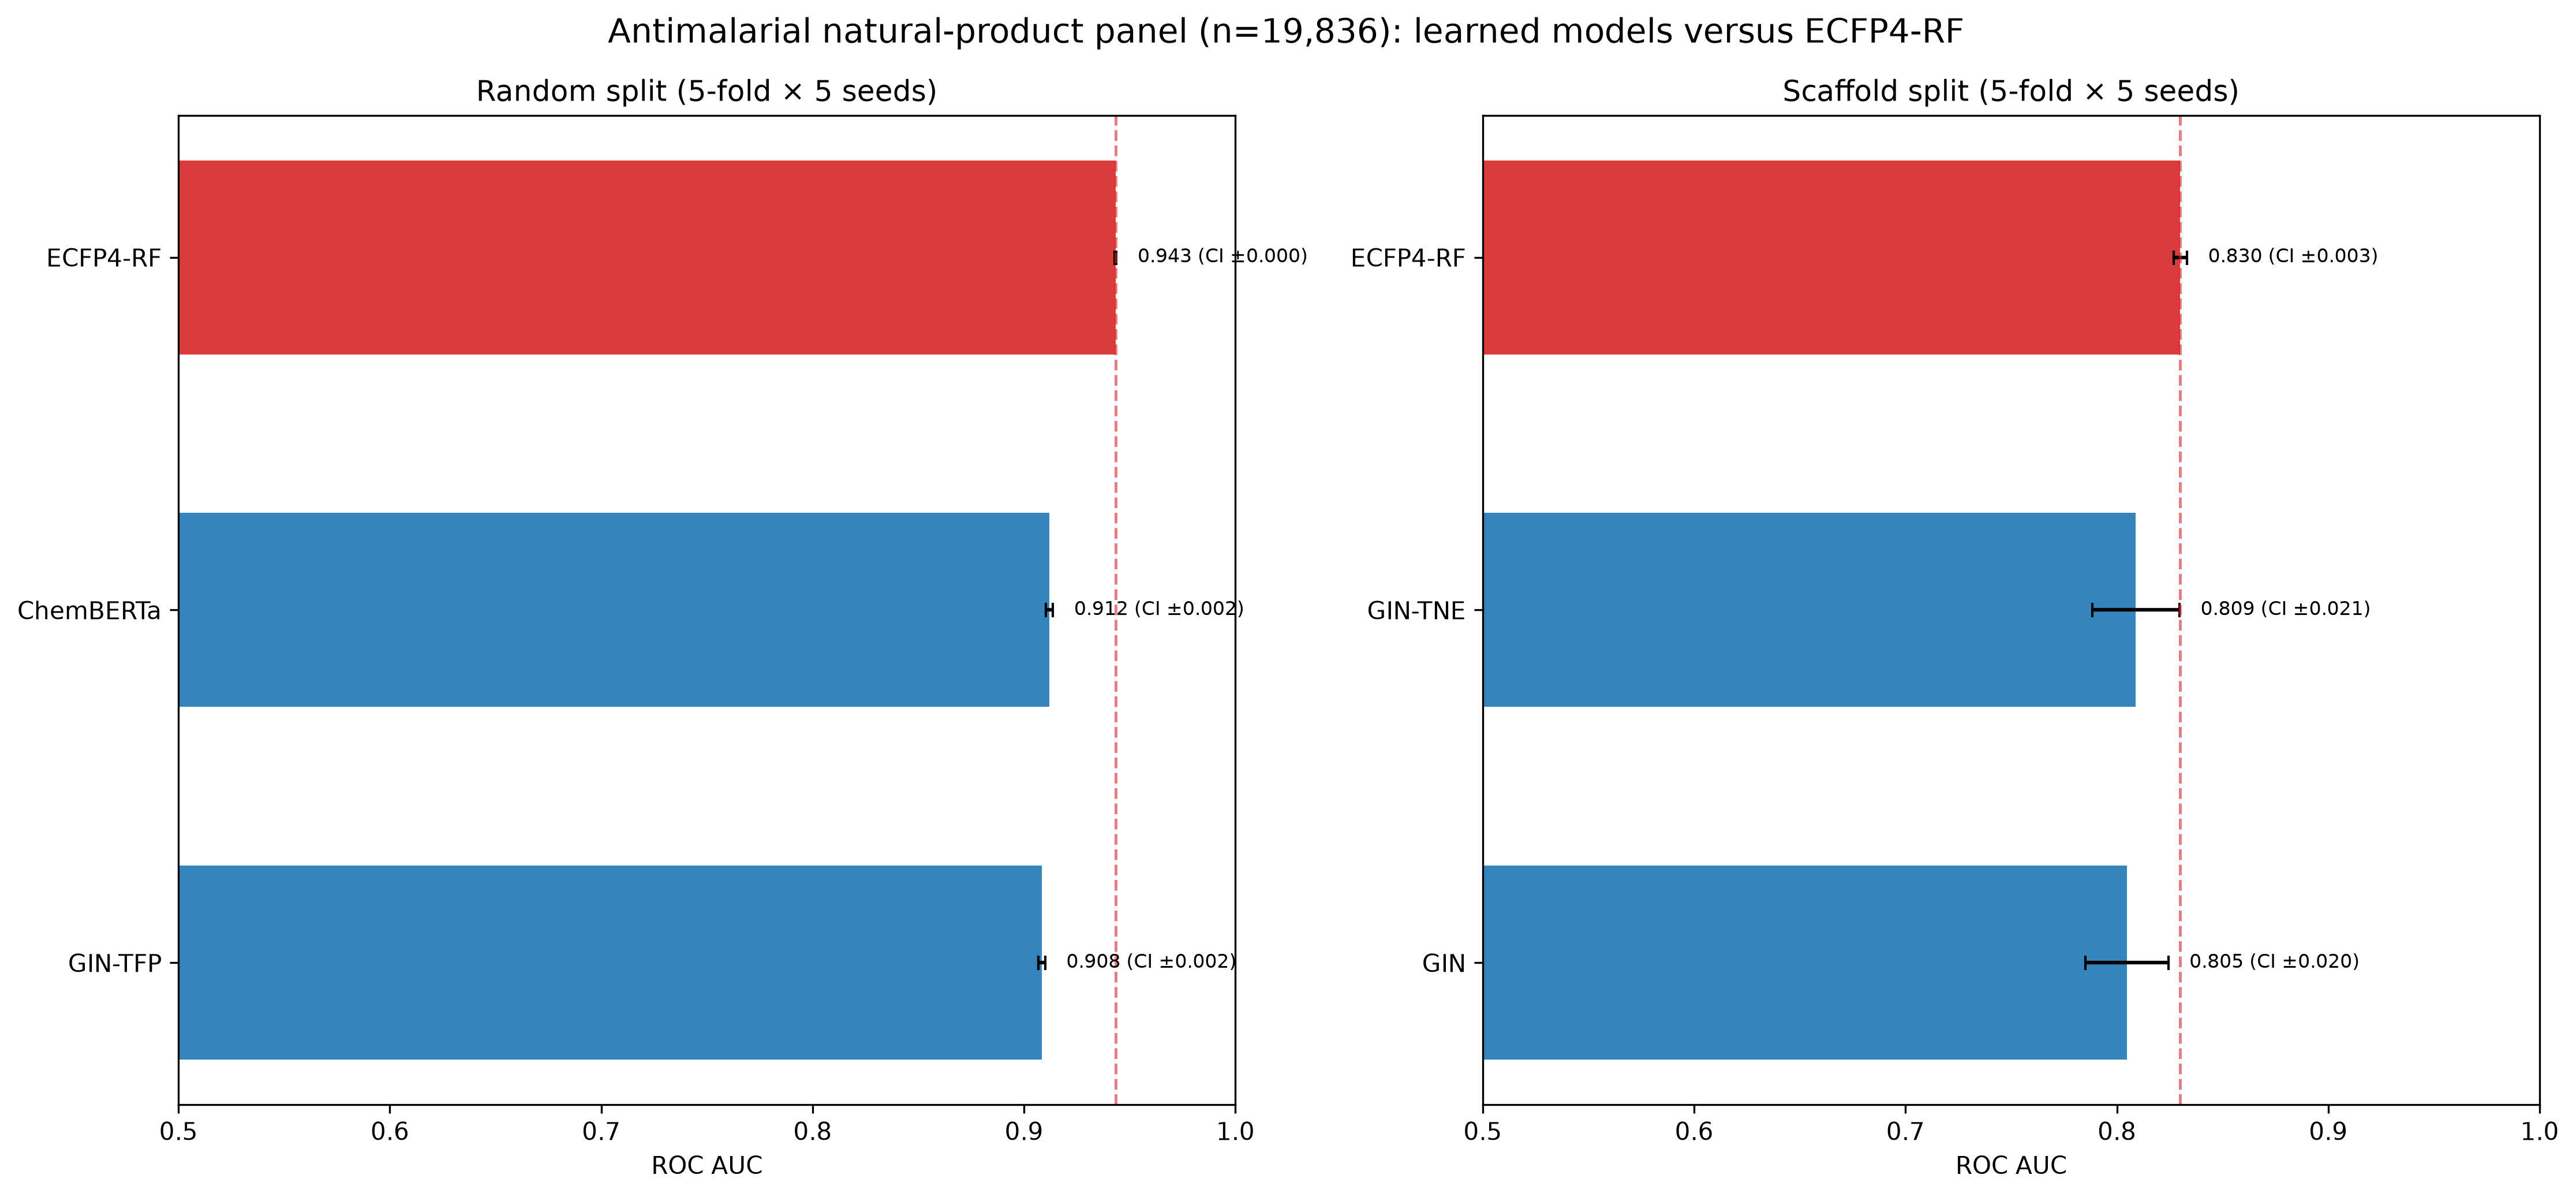
\includegraphics[width=0.98\textwidth]{p5_auc_benchmark.png}
\caption{Mean test ROC AUC with \qty{95}{\percent} confidence intervals computed from five per-seed means (each mean aggregates five fold-level test AUCs), shown for random (left) and scaffold (right) splits. The underlying analysis contains \num{25} fold--seed replicates per model and split. Bar annotations report the mean followed by the CI half-width. The ECFP4--RF baseline (red) is not exceeded by any tested GNN or transformer arm.}
\label{fig:benchmark}
\end{figure}

The available validation trajectories show how checkpoint selection proceeded over \num{50} training epochs with an early-stopping patience of \num{10}; these curves describe optimization behaviour rather than establishing the absence of over-fitting (\cref{fig:learning_curves}).

\begin{figure}[t]
\centering
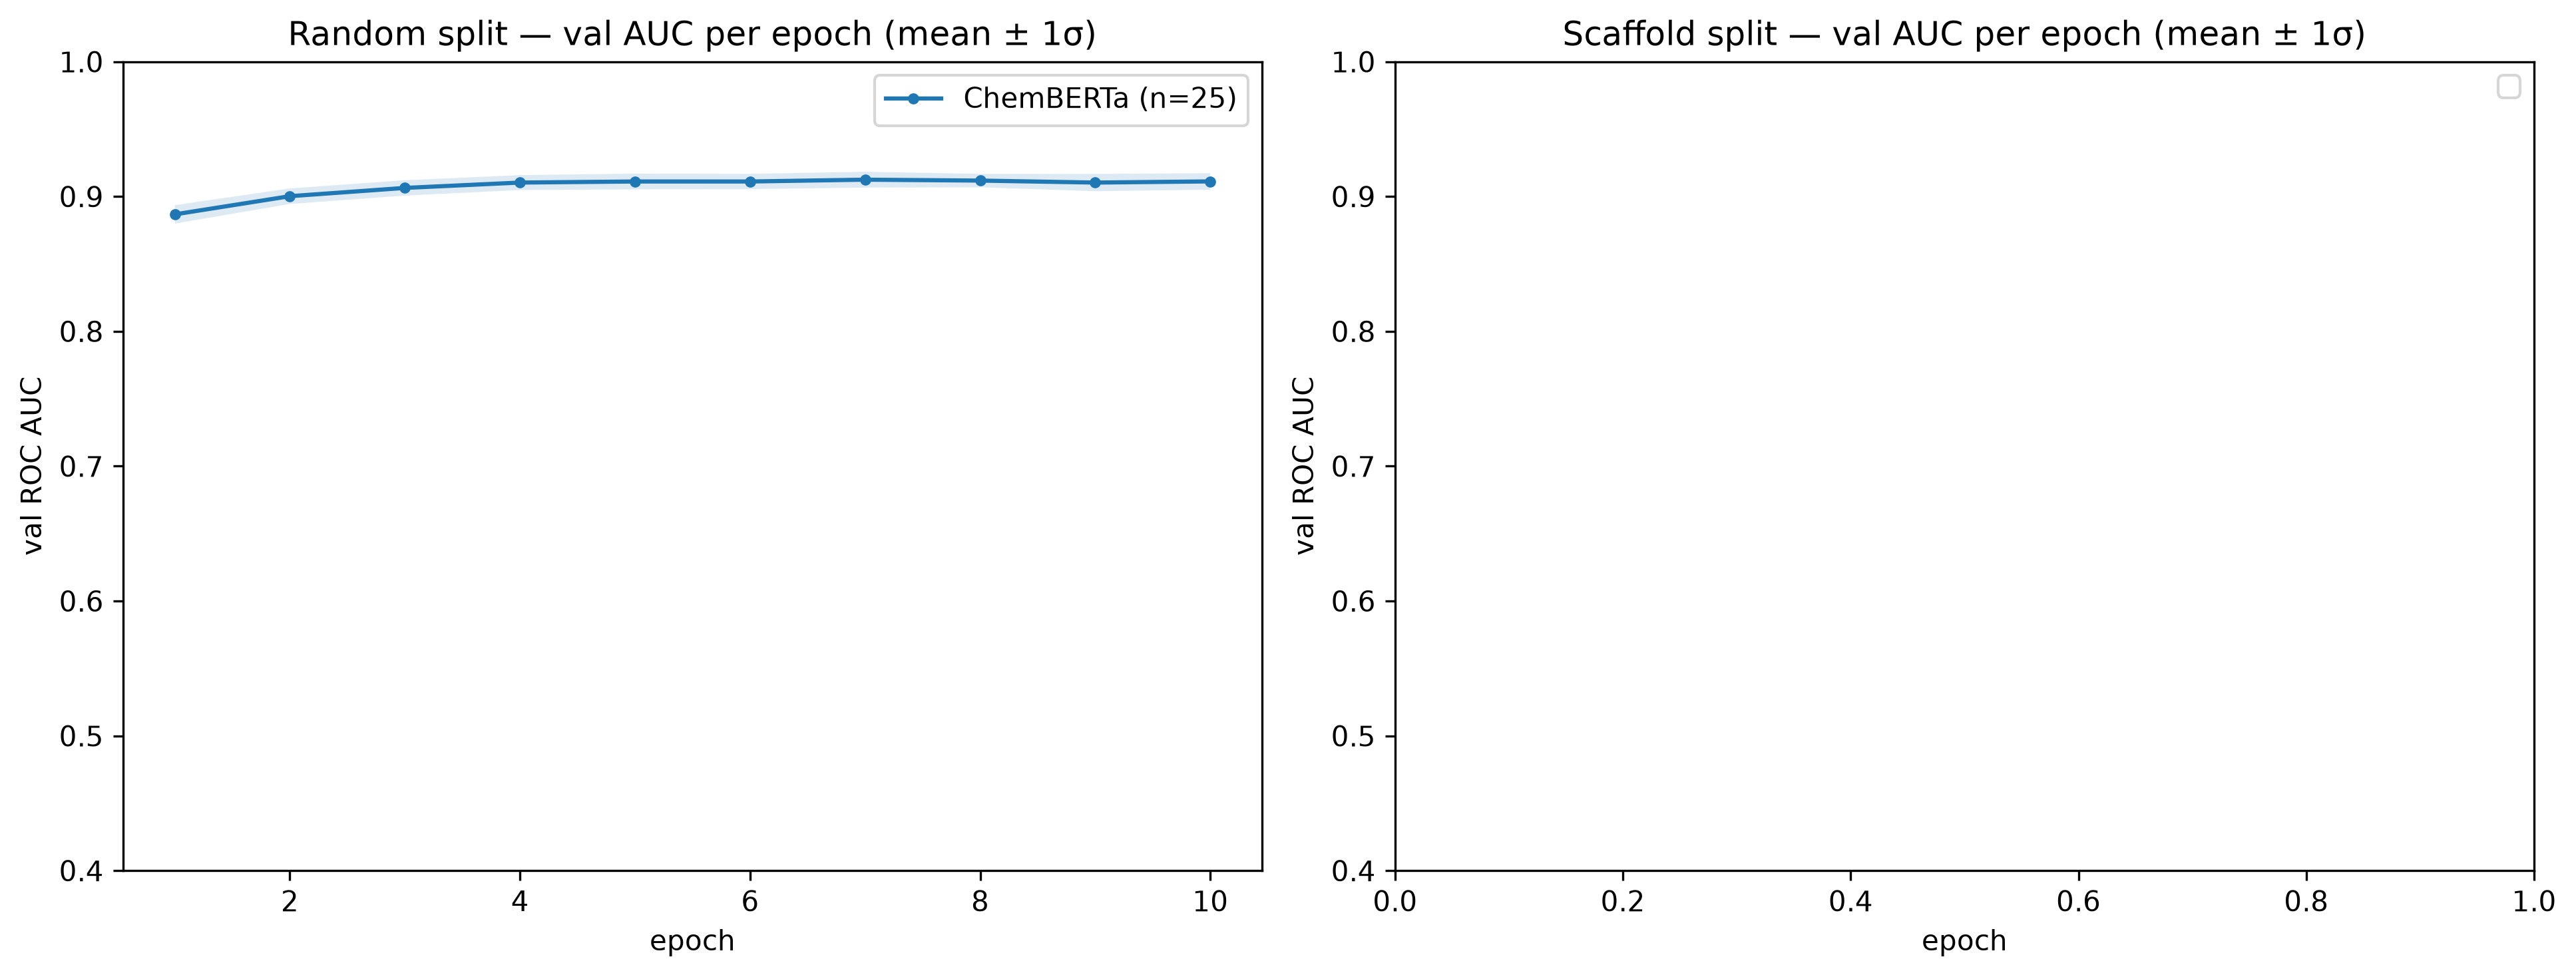
\includegraphics[width=0.95\textwidth]{p5_learning_curves.png}
\caption{Validation ROC AUC trajectories used for checkpoint selection. Curves are available for GIN under random and scaffold splits, GIN--TFP and GIN--TNE under both random and scaffold splits, and ChemBERTa under both random and scaffold splits; each available arm contains five folds repeated over five seeds. Early stopping with patience \num{10} selects the checkpoint before test evaluation.}
\label{fig:learning_curves}
\end{figure}

\subsection{H3: topological features remain visible in the fusion head despite the ranking deficit}

Even when predictive gains are absent, learned fusion weights carry structure that can be examined descriptively. We compute a \emph{salience} score for each descriptor dimension as the mean absolute weight in the fusion projection layer ($\mathrm{head}_0$) over the \num{25} replicates. For the TFP fusion (\num{78} dimensions: \num{33} homology-dimension-0, \num{25} persistent-image, \num{20} Betti), the \emph{persistent-image block (dims \num{33}--\num{57}) has the largest raw mean projection-weight magnitude} (\num{0.0790}) versus homology-0 (\num{0.0485}) and Betti (\num{0.0547}) blocks; the top five dimensions are persistent-image (\num{42}, \num{43}, \num{52}, \num{53}, \num{54}). For the TNE fusion (\num{192} dimensions) the top dimensions are \num{68}, \num{43}, \num{92}, \num{66}, \num{165}, and the top-\qty{10}{\percent} of dimensions account for \qty{17.3}{\percent} of total salience (moderate sparsity).

This pattern indicates that topological descriptors are used by the fusion head, but it does not establish feature necessity or causal relevance. On this panel, the descriptor signal does not translate into a ranking advantage over fingerprints. Thus, projection-weight salience and predictive ranking should be treated as complementary, not interchangeable, summaries.

\begin{figure}[t]
\centering
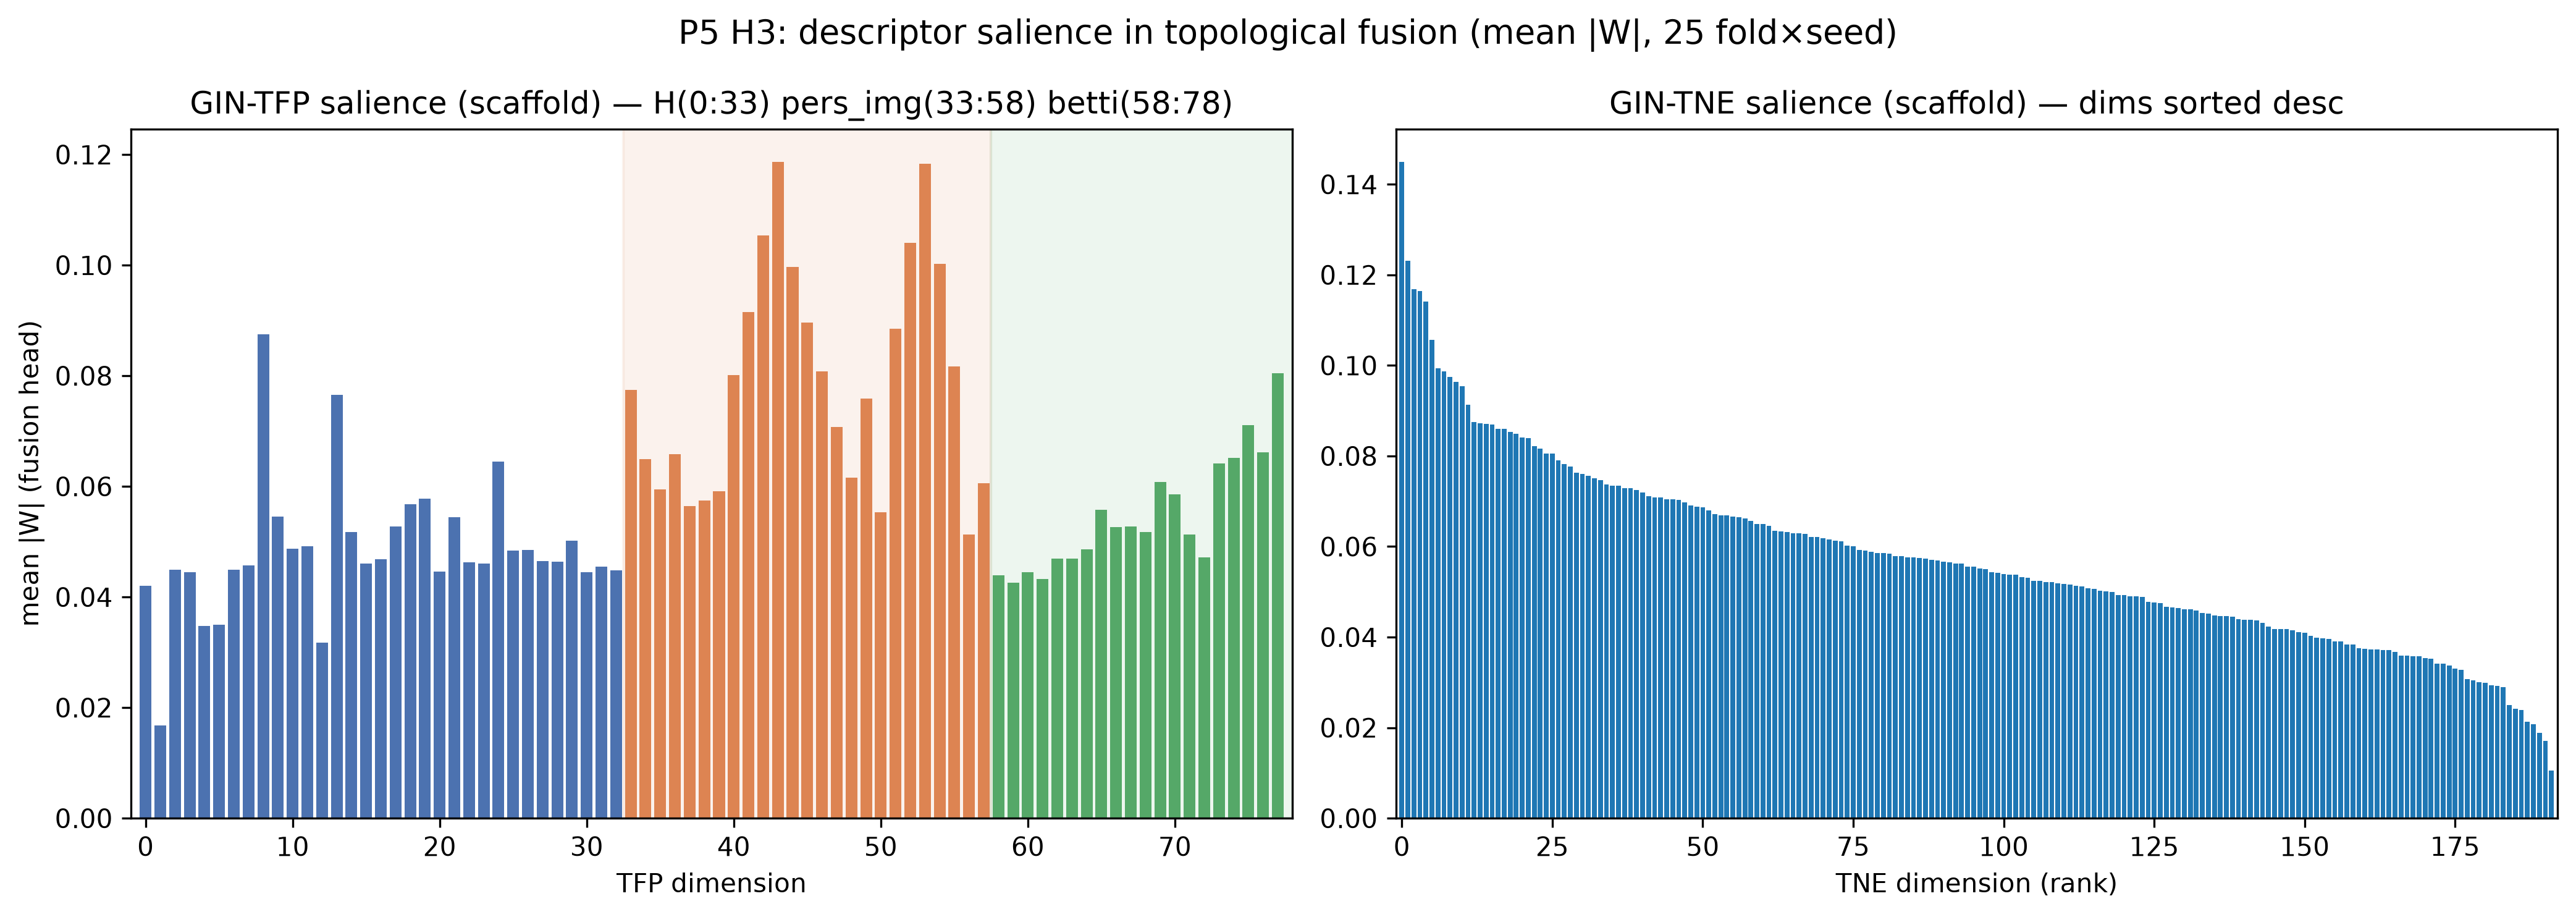
\includegraphics[width=0.98\textwidth]{p5_salience.png}
\caption{Descriptive projection-weight salience in the topological fusion heads under the scaffold split. Values are mean raw $|W|$ across \num{25} fold--seed replicates. Left: TFP (\num{78} dimensions), partitioned into homology-0 (dims \num{0}--\num{32}), persistent-image (dims \num{33}--\num{57}), and Betti (dims \num{58}--\num{77}); the persistent-image block has the largest raw weight magnitude. Right: TNE (\num{192} dimensions), shown in descending order. Weight magnitude is interpreted descriptively and is not a causal attribution.}
\label{fig:salience}
\end{figure}

\section{Discussion}

The three questions yield a coherent conclusion: learned representations do not exceed ECFP4 under either split; topological fusion narrows the scaffold gap modestly but does not close it; and persistent-image dimensions remain salient in the fusion head without yielding a ranking advantage. Predictive utility and interpretive visibility are separable properties.

\subsection{The verdict is scale-independent and panel-specific}

The primary result is that the tested pretrained and graph-based models did not improve ROC AUC over ECFP4--RF on this panel, including under scaffold-held-out testing. This conclusion is supported by repeated evaluation, paired comparisons on the five per-seed means, and correction for multiplicity. The transformer result depends critically on fold-independent weight initialization: pretrained weights were reset at the beginning of every fold so that fine-tuning could not transfer between test folds. Future molecular-benchmark studies should state explicitly whether pretrained weights are reset for every fold.

\subsection{Why fingerprints hold: representation--task alignment}

The consistent ECFP4 advantage is best explained by representation--task alignment. ECFP4 encodes local substructure environments; for structurally related natural products, local SAR is the dominant signal, and tree ensembles exploit it efficiently with few thousand labels \citep{ecfp_2010}. Learned graph representations require more data to recover the same local patterns and generalize to scaffold-held-out series only partially \citep{benchmark_pretrained_2025}. This is consistent with the medicinal-chemistry view that fingerprints plus random forests remain an effective early-stage tool \citep{learning_mol_repr_2020}. The counterpoint that graph models can be made competitive by training them \emph{on} fingerprints is instructive: ECFP-pretrained GNNs improve out-of-distribution performance on homogeneous ADMET tasks but still underperform on heterogeneous endpoints such as binding affinity \citep{ecfp_pretrained_2026}---mirroring the fingerprint-centric explanation, since pretraining transfers the very substructure knowledge fingerprints encode. Our H3 result adds a nuance: topological descriptors are not uninformative---they carry interpretable geometric signal---but their marginal ranking contribution is small on this panel.

\subsection{Relation to prior antimalarial modelling}

The molecular collection and fingerprint implementation were previously characterized in a quantum-representation benchmark \citep{temgoua2027quantum}. That study found no statistically detectable advantage of the simulated quantum kernel over a tuned radial-basis kernel; the present analysis tests a different question---whether graph or sequence models improve activity ranking on the same chemical collection. Molecular-dynamics studies of selected antimalarial leads have additionally examined resistance-associated targets and mutations \citep{temgoua2027md}; those simulations provide biological context but are not labels or validation data for the present benchmark. Topological descriptors are used descriptively by the fusion head, but none of the tested learned representations improves ROC AUC over ECFP4--RF.

\subsection{Practical recommendations}

For comparable antimalarial NP panels, ECFP4--RF is a strong first-line baseline: it is computationally inexpensive and outperformed every tested neural arm. Graph and sequence models should be evaluated against this baseline under scaffold-held-out testing rather than assumed to improve from model scale alone. Transformer studies should reset pretrained weights for every fold and record the initialization protocol. Topological or tensor-network descriptors can be examined as complementary descriptive features, but their inclusion should not be interpreted as evidence of improved ranking without a paired comparison.

\subsection{Limitations}

Our panel, while curated and clinically motivated, is a single binary-activity collection assembled from screening data. To test whether the verdict is specific to these computational labels, we repeated the ECFP4--RF versus GIN comparison on a disjoint ChEMBL-derived activity benchmark built from recorded IC\textsubscript{50}/EC\textsubscript{50} activities against \emph{Plasmodium falciparum} (target CHEMBL364, \num{22267} molecules after excluding \num{180} compounds overlapping the P5 panel; actives at pChEMBL $\geq \num{6.0}$). The fingerprint baseline again wins: ECFP4--RF \num{0.9190} $\pm$ \num{0.0004} versus GIN \num{0.8843} $\pm$ \num{0.0021} under the scaffold split ($\Delta = +\num{0.035}$, paired $p < \num{0.0001}$). Because this external analysis used an independently constructed split rather than the frozen internal fold files, it is a transfer analysis rather than a strict replication; it nevertheless indicates that the ordering is not unique to the eOS80CH screening labels.

The GNN and fusion models use a single-layer prediction head and fixed hyperparameters (hidden dimension \num{128}, \num{50} epochs, patience \num{10}); alternative architectures or tuning could reduce the observed gap. ChemBERTa was fine-tuned with a fixed learning schedule rather than per-task optimization. The GIN uses 2D molecular graphs without conformational information; 3D-equivariant architectures may perform differently on tasks for which shape is important \citep{rollins2024molprop}. The salience measure (mean absolute projection weight) captures correlation between descriptor dimensions and the predictive head, not causation; more sophisticated methods (e.g., integrated gradients, SHAP) would be needed to establish which features are truly necessary. Finally, the scaffold split is a proxy for novelty; a recent structural-frontier analysis shows that splits reserving the sparsest, physicochemically remote scaffold groups inflate error further on ADMET tasks \citep{scaffold_frontier_2026}; harder forms of novelty pose an even steeper generalization test.

\section{Conclusions}

The central question was whether larger graph and sequence models improve activity prediction beyond ECFP4 when chemical scaffolds are held out. On a frozen panel of \num{19836} African antimalarial natural products, ECFP4--RF outperformed the tested GIN, topological-fusion GNNs, and fine-tuned ChemBERTa transformer under both random and Bemis--Murcko scaffold cross-validation. Under the scaffold split, the hierarchy was ECFP4--RF (\num{0.8300}) > GIN--TFP (\num{0.8138}) > GIN--TNE (\num{0.8090}) > GIN (\num{0.8047}) > ChemBERTa (\num{0.7867}); all four learned arms were significantly below the fingerprint baseline after multiplicity correction. The external ChEMBL-derived analysis showed the same ordering, while remaining an observational transfer analysis of thresholded activity records. Persistent-image dimensions had the largest projection-weight salience in the fusion head, indicating that topological features carry interpretable geometric signal even though they do not improve ranking.

Three practical implications follow. First, ECFP4--RF should be treated as the default baseline for antimalarial NP panels; any claimed improvement from a neural architecture must demonstrate a statistically significant gain under scaffold-held-out testing. Second, topological and tensor-network descriptors carry interpretable geometric signal that can be examined descriptively, but their inclusion in a fusion architecture does not automatically translate into a ranking advantage. Third, the fold-independent transformer initialization protocol reported here should be adopted in future molecular-benchmark studies to prevent inflated cross-validation estimates. Experimental validation on prospectively synthesised candidates remains necessary to test whether the computational ranking predicts biological activity.

\section{List of Abbreviations}

\textbf{ECFP4:} extended-connectivity fingerprint, radius \num{2}; \textbf{RF:} random forest; \textbf{GNN:} graph neural network; \textbf{GIN:} graph isomorphism network; \textbf{TFP:} topological fingerprint; \textbf{TNE:} tensor-network embedding; \textbf{ROC AUC:} receiver-operating-characteristic area under the curve; \textbf{CV:} cross-validation; \textbf{NP:} natural product; \textbf{ADMET:} absorption, distribution, metabolism, excretion, toxicity.

\section{Methods}

\subsection{Data and panel}

We use a frozen panel of \num{19836} molecules with binary antimalarial activity labels from the eOS80CH screening collection, curated and deduplicated by canonical SMILES as described previously \citep{temgoua2026antimalarial}. Features are ECFP4 (\num{2048}-bit Morgan radius-\num{2}), a \num{78}-dimensional topological fingerprint (TFP; persistent homology, persistent images, and Betti descriptors), and \num{192}-dimensional tensor-network embeddings (TNE). All features are aligned to the same molecule index.

\subsection{Splits}

Two protocols were evaluated, each with five folds repeated over five seeds (\num{25} fold--seed replicates). (i) \emph{Random}: stratified five-fold cross-validation. (ii) \emph{Scaffold}: molecules were grouped by Bemis--Murcko scaffold before fold assignment; the held-out test scaffolds are disjoint from the training scaffolds. Validation molecules were sampled from the non-test portion and therefore can share scaffolds with training molecules; early stopping consequently assesses optimization on the training chemical distribution, whereas the held-out test fold provides the scaffold-shift estimate. The split indices are released with the study.

\subsection{Models}

\textbf{ECFP4--RF}: scikit-learn RandomForest on ECFP4, the reference baseline. \textbf{GIN}: graph isomorphism network (\num{128} hidden units, mean-pooling readout, single head) trained on molecular graphs (atom/edge features from RDKit). We select GIN as the representative GNN architecture following MolGraphBench \citep{guo_ding_2026}, which identified GIN as the optimal GNN for molecular regression across multiple benchmarks; GCN, GAT, and GraphSAGE were evaluated in that study and did not consistently outperform GIN, so we omit them to avoid redundancy. \textbf{GIN--TFP / GIN--TNE}: the same GIN with the topological descriptor vector concatenated at the head ($\mathrm{head}_0 = \mathrm{Linear}(\num{128} + n_{desc} \to \num{128})$), enabling the salience attribution. \textbf{ChemBERTa}: pretrained SMILES transformer, fine-tuned with cross-entropy and independent pretrained-weight initialization for every fold. All deep models trained on a single NVIDIA RTX A4000 GPU with AdamW, early stopping on validation AUC (patience \num{10} of \num{50} epochs), and best-val checkpoint selection.

\subsection{Fold-independent transformer initialization}

For each fold, the pretrained ChemBERTa state is restored before fine-tuning, so no fold receives weights updated on another fold. This independence is essential because cross-fold weight transfer can inflate test AUCs by up to \num{0.15}. All transformer results use independent fold initialization and the same training schedule.

\subsection{Statistics}

Per model and split, we retain the \num{25} fold--seed AUCs and summarize them as five per-seed means, each averaging the five fold-level test AUCs. Model-versus-baseline comparisons use paired $t$-tests on these five per-seed means ($df=4$), rather than treating the \num{25} fold--seed values as independent observations. Table values are mean $\pm$ SD across the five per-seed means; the raw two-sided $p$-values are corrected with Benjamini--Hochberg separately across the four scaffold comparisons and the four random comparisons. Under scaffold this yields adjusted $p$-values of \num{0.0330} (GIN), \num{0.0330} (GIN--TFP), \num{0.0378} (GIN--TNE), and \num{0.0002} (ChemBERTa); under random all four arms remain below the baseline after correction. The significance threshold is $\alpha=\num{0.05}$ and effect sizes are reported as mean differences. Salience is aggregated across the \num{25} replicates as the per-dimension mean absolute projection weight.

\section{Availability of data and materials}

All code, frozen splits (random and scaffold, five seeds each), per-fold results, salience data, figure scripts, and the \num{19836}-molecule panel are available under the MIT licence in the public GitHub repository (\url{https://github.com/NanaEngo/Malaria_codesV2}). Trained checkpoints and feature tables are included; reproducibility is supported by the frozen split files and the pinned environment.

\noindent\textbf{Secondary scaffold-only replication.} An independent scaffold evaluation (five folds $\times$ five seeds) produced all \num{25} fold--seed records and a mean ROC AUC of $\num{0.7908} \pm \num{0.0058}$ when summarized across five per-seed means; the primary scaffold estimate was $\num{0.7867} \pm \num{0.0054}$ under the same summary. The primary random-split estimate was $\num{0.9121} \pm \num{0.0012}$; no independent random-split replication was performed.

\section{Author contributions}

MVST conceived the study, designed the benchmark protocol, implemented the GNN/transformer pipelines, and wrote the manuscript. All authors contributed to data analysis, reviewed the results, and approved the final version. (CRediT roles and full author affiliations are listed on the title page.)

\section{Competing interests}

The authors declare no competing interests.

\section{Funding}

This research received no specific grant from any funding agency in the public, commercial, or not-for-profit sectors.

\section{Ethics approval and consent to participate}

Not applicable. This study is entirely computational and uses publicly available chemical databases and in-silico activity predictions; no human or animal subjects or patient data were involved.

\section{Consent for publication}

Not applicable. No individual person's data (including images, videos, or identifiable details) appear in this manuscript.

\section{Use of Artificial Intelligence}

During the preparation of this work the authors used AI assistants to support code development and data analysis scripting. The authors reviewed and edited all AI-assisted output and take full responsibility for the content of this article. No generative AI tool is listed as an author. Computational results, statistical analyses, and all quantitative claims were generated and verified by the authors; the public repository contains the currently released artefacts.

\section{Acknowledgements}

The authors acknowledge the University of Yaoundé I high-performance computing facility used for the GPU and CPU calculations.

\section*{References}
\bibliographystyle{unsrtnat}
\bibliography{Bibliography_P5}

\end{document}
